\section*{GBM}

Gradient Boosting Method is an agorithm that is part of \hyperref[sec:ensemble-methods]{ensemble methods}.

There are many different implementation of this algorithm; the below one (src: Wikipedia) is one of the most generic and understandable.

\begin{center}
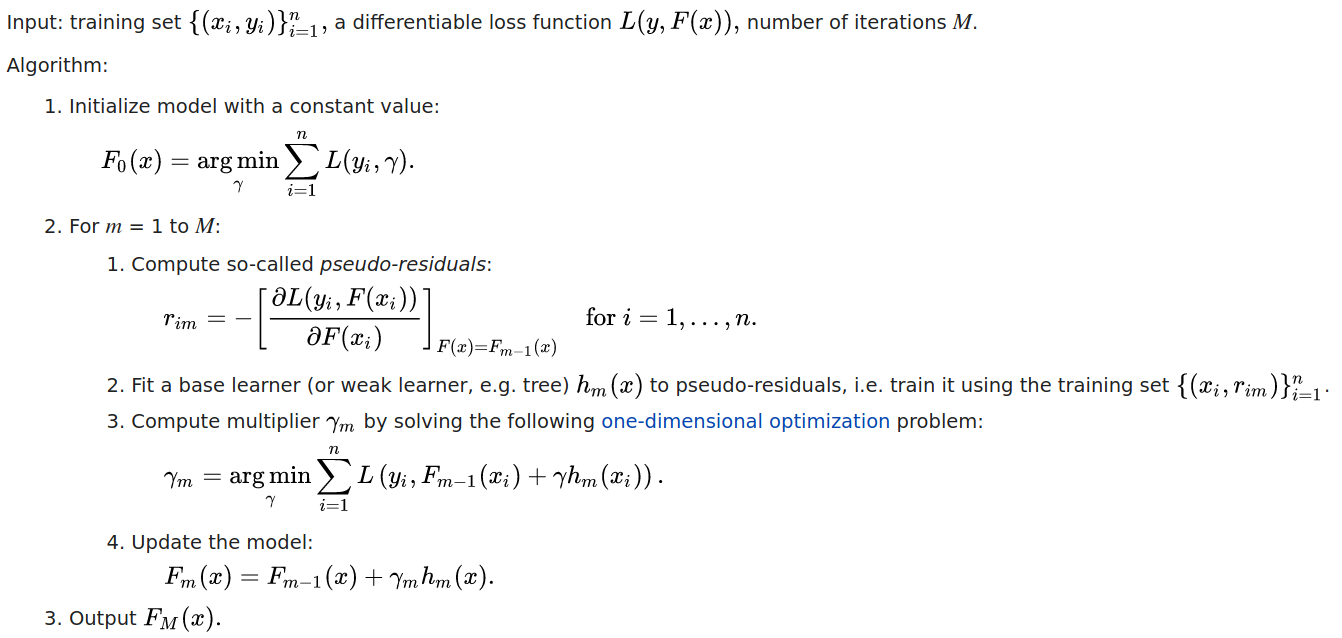
\includegraphics[scale=0.3]{GBM_algo.png}
\end{center}

\underline{Step 1: initialize model with constant value}

$$F_0 = \underset{\hat y}{argmin} \Sigma_{i=1}^n \mathcal{L}(y,\hat y)$$

We note that $\hat y$ is constant and doesn't depend on $i$. Consequently, optimizing this equation using SE as loss function will lead to $\hat y = \bar y$:

Note: $MSE := \frac{1}{n}\Sigma_{i=1}^n (y_i - \hat y)^2$ thus $\mathcal{L}: (y,\hat y) \to (y-\hat y)^2$ but we usually choose $\mathcal{L}: (y,\hat y) \to \frac{1}{2}(y-\hat y)^2$\\

$\frac{\partial MSE}{\partial \hat y} = 0$

=> $\frac{2}{n}(y_1 - \hat y) + ... + \frac{2}{n}(y_n - \hat y) = 0$

=> $\hat y = \Sigma_{i=1}^n \frac{y_i}{n} = \bar y$ \\

\underline{Step 2: loop on the number of estimators} \\

\textit{Pseudo-residuals} \\

$$res = - \frac{\partial \mathcal{L}}{\partial \hat y}$$

The gradient of the loss function is $\frac{\partial \mathcal{L}}{\partial \hat y} = -(y - \hat y)$

Residuals as seen in linear regression are typically written as such: $res = y - \hat y$. Thus, gradient boosting uses negative residuals, also called \textbf{pseudo-residuals}. 

Note: pseudo-residuals are just the derivatives of the loss function; that's why we call it \textbf{gradient} boosting. \\

\textit{Fit a weak learner} \\

\lstset{language=Python}
\lstset{frame=lines}
\lstset{caption={Fit base learner}}
\lstset{label={lst:code_direct}}
\lstset{basicstyle=\footnotesize}
\begin{lstlisting}
h = tree.fit(x, res)
\end{lstlisting}

Weak learners (see definition in \hyperref[sec:adaboost]{Adaboost} section) used in gradient boosting are typically decision trees. These learners are trained on residuals. \\

\textit{Compute the gradient step} \\



\textit{Update the function} \\

\underline{Step 3: Output the function} \\


Implementation from scratch - comments

Parameters to optimize

\vspace{5mm}